% Chương 4
\chapter[\MakeUppercase{Tổ chức và truy xuất tri thức cho RAG bằng kho vector và đồ thị tri thức}]{Tổ chức và truy xuất tri thức cho RAG bằng kho vector và đồ thị tri thức}
\label{ch:chuong4}

Chương này nhắc lại cơ sở lý thuyết về RAG (mục~\ref{sec:ly-thuyet-rag}), rồi mô tả cơ sở tri thức mà chatbot truy xuất (mục~\ref{sec:nguon-kb}) và luồng truy xuất chính của chatbot (mục~\ref{sec:luong-truy-xuat}). Mọi kết quả truy xuất chỉ hỗ trợ lập luận, không phải chẩn đoán y khoa.

\section{Cơ sở lý thuyết về RAG}
\label{sec:ly-thuyet-rag}

\subsection{Hạn chế của mô hình ngôn ngữ lớn khi dùng độc lập}

Mô hình ngôn ngữ lớn (LLM) sinh câu trả lời từ tri thức đã học trong tham số. Cách này có bốn hạn chế khi áp dụng vào y khoa:
\begin{itemize}
  \item \textbf{Tri thức cố định:} mô hình chỉ biết nội dung có trong dữ liệu huấn luyện; muốn cập nhật phải huấn luyện lại.
  \item \textbf{Nội dung sai nhưng trôi chảy:} mô hình có thể bịa chi tiết (hiện tượng ``ảo giác'' -- hallucination) mà văn phong vẫn tự tin.
  \item \textbf{Không nêu nguồn:} người đọc không kiểm tra được câu trả lời dựa trên tài liệu nào.
  \item \textbf{Thiếu tri thức riêng:} giáo trình đã chọn và ca bệnh của cơ sở không nằm trong tham số của mô hình.
\end{itemize}

\subsection{Nguyên lý của RAG}

Truy xuất tăng cường sinh văn bản (RAG -- Retrieval-Augmented Generation) tách việc ``biết'' khỏi việc ``viết''. Tri thức nằm trong một kho ngoài mô hình. Với mỗi câu hỏi, hệ thống tìm các đoạn liên quan trong kho, đưa chúng vào đầu vào của LLM, rồi để LLM viết câu trả lời dựa trên các đoạn đó. Gọi $q$ là câu hỏi, $\mathcal{K}$ là kho tri thức, hàm $R$ là bước truy xuất và $G$ là LLM, câu trả lời $\hat{y}$ được tạo như sau:
\begin{equation}
\mathcal{C} = R(q, \mathcal{K}), \qquad \hat{y} = G(q, \mathcal{C})
\label{eq:rag-tong-quat}
\end{equation}
Trong đó, $\mathcal{C}$ là tập $k$ đoạn được chọn. Vì $\mathcal{C}$ đi kèm vị trí trong tài liệu gốc nên câu trả lời có thể ghi nguồn.

Một hệ thống RAG có hai giai đoạn (hình~\ref{fig:rag-hai-giai-doan}). Giai đoạn nạp tri thức chạy trước, một lần cho mỗi tài liệu. Giai đoạn truy vấn chạy ở mỗi câu hỏi.

\begin{figure}[H]
\centering
\begin{tikzpicture}[
    node distance=0.5cm,
    rbox/.style={rectangle, draw=black!70, thick, rounded corners=3pt, align=center, inner sep=3pt, font=\footnotesize, minimum width=2.4cm, minimum height=0.9cm},
    rstep/.style={rbox, fill=gray!10},
    rstore/.style={rbox, fill=blue!10, draw=blue!75!black},
    rgen/.style={rbox, fill=green!12, draw=green!70!black},
    arr/.style={-{Stealth[scale=1.1]}, thick}
]
    \node (d1) [rstep] {Tài liệu\\nguồn};
    \node (d2) [rstep, right=of d1] {Chia\\thành đoạn};
    \node (d3) [rstep, right=of d2] {Mã hóa\\(embedding)};
    \node (d4) [rstore, right=of d3] {Kho tri thức\\(vector, đồ thị)};
    \node (q1) [rstep, below=1.7cm of d1] {Câu hỏi};
    \node (q2) [rstep, right=of q1] {Truy xuất\\đoạn liên quan};
    \node (q3) [rstep, right=of q2] {Ghép\\ngữ cảnh};
    \node (q4) [rgen, right=of q3] {Mô hình\\ngôn ngữ};
    \node (q5) [rgen, right=of q4] {Câu trả lời\\kèm nguồn};
    \node [font=\small\bfseries, anchor=south west] at ($(d1.north west)+(0,0.15)$) {(a) Giai đoạn nạp tri thức};
    \node [font=\small\bfseries, anchor=south west] at ($(q1.north west)+(0,0.15)$) {(b) Giai đoạn truy vấn};
    \draw [arr] (d1) -- (d2);
    \draw [arr] (d2) -- (d3);
    \draw [arr] (d3) -- (d4);
    \draw [arr] (q1) -- (q2);
    \draw [arr] (q2) -- (q3);
    \draw [arr] (q3) -- (q4);
    \draw [arr] (q4) -- (q5);
    \draw [arr, dashed] (d4.south) -- ++(0,-0.75) -| ([xshift=-0.35cm]q2.north east);
\end{tikzpicture}
\caption{Hai giai đoạn của hệ thống RAG}
\label{fig:rag-hai-giai-doan}
\end{figure}

RAG vẫn có giới hạn: nếu truy xuất bỏ sót đoạn cần thiết hoặc kho tri thức sai, câu trả lời sai dù có dẫn nguồn; LLM cũng có thể diễn giải sai đoạn đã cho. Trong lĩnh vực da liễu, kết quả của RAG là gợi ý hỗ trợ, không phải chẩn đoán y khoa.

\subsection{Các thành phần RAG trong hệ thống}

Một hệ thống RAG gồm các thành phần: chia đoạn (chunking), mã hóa (embedding), kho tri thức, truy xuất, xếp hạng lại (reranking) và sinh có căn cứ. Hai mục sau mô tả cách hệ thống hiện thực các thành phần này:
\begin{itemize}
  \item \textbf{Mục~\ref{sec:nguon-kb}:} nguồn tri thức và cách đưa vào kho, gồm chia đoạn, mã hóa và lưu trữ.
  \item \textbf{Mục~\ref{sec:luong-truy-xuat}:} các luồng truy xuất, gồm tìm kiếm ngữ nghĩa, từ khóa, đồ thị, luồng hỗn hợp kết hợp ba hướng này và xếp hạng lại.
\end{itemize}

Thành phần còn lại, sinh có căn cứ, do chatbot thực hiện và được trình bày ở Chương~\ref{ch:chuong5}.

\section{Nguồn tri thức của chatbot da liễu}
\label{sec:nguon-kb}

\subsection{Ba nguồn tri thức và nơi lưu trữ}

Chatbot truy xuất từ ba nguồn: giáo trình số hóa, ca bệnh đã kết luận và đồ thị tri thức có sẵn (PrimeKG, DermO). Đoạn văn của giáo trình và ca bệnh lưu trong Qdrant (cơ sở dữ liệu vector). Đồ thị lưu trong Neo4j (cơ sở dữ liệu đồ thị), gồm đồ thị có sẵn và quan hệ trích được từ giáo trình.


\begin{table}[H]
\centering
\caption{Các nguồn tri thức và cách truy xuất}
\label{tab:nguon-kb}
\small
\begin{tabular}{|p{3.2cm}|p{2.2cm}|p{5.6cm}|p{3.0cm}|}
\hline
\textbf{Nguồn} & \textbf{Kho} & \textbf{Nội dung} & \textbf{Cách truy xuất} \\ \hline
Giáo trình số hóa (ba sách) & Qdrant\newline Neo4j & Đoạn (chunk) cắt theo mục lục, kèm sách, mục, số trang; quan hệ bệnh -- thuốc -- triệu chứng trích từ sách, kèm câu trích và số trang & Tìm kiếm hỗn hợp, có cả luồng đồ thị (mục~\ref{sec:luong-hon-hop} và~\ref{sec:luong-do-thi}) \\ \hline
Ca bệnh đã kết luận & Qdrant & Báo cáo kết luận do bác sĩ lập: chẩn đoán, triệu chứng, dặn dò, ảnh & Tìm ca tương tự theo văn bản hoặc theo ảnh \\ \hline
Đồ thị có sẵn: PrimeKG, DermO & Neo4j & Quan hệ y sinh và ontology da liễu & Truy vấn theo ý định (mục~\ref{sec:truy-xuat-do-thi}) \\ \hline
\end{tabular}
\end{table}

\begin{figure}[H]
\centering
\begin{tikzpicture}[
  font=\small, >=Stealth,
  src/.style={rectangle, rounded corners=3pt, draw=gray!70, fill=gray!12, minimum width=3.4cm, minimum height=0.9cm, align=center},
  store/.style={rectangle, rounded corners=3pt, draw=blue!55!black, fill=blue!10, minimum width=2.8cm, minimum height=1.0cm, align=center},
  bot/.style={rectangle, rounded corners=3pt, draw=orange!70!black, fill=orange!12, minimum width=2.2cm, minimum height=1.2cm, align=center},
  lab/.style={font=\scriptsize, midway, sloped, above}]
\node[src] (report) at (0,3) {Báo cáo kết luận\\của bác sĩ};
\node[src] (pdf) at (0,0.4) {PDF giáo trình};
\node[src] (kg) at (0,-2.2) {PrimeKG, DermO};
\node[store] (qdrant) at (5.6,2.2) {Qdrant\\(vector)};
\node[store] (neo) at (5.6,-1.6) {Neo4j\\(đồ thị)};
\node[bot] (chat) at (10.4,0.3) {Chatbot};
\draw[->] (report) -- node[lab] {văn bản + vector} (qdrant);
\draw[->] (pdf) -- node[lab] {chunk + vector} (qdrant);
\draw[->] (pdf) -- node[lab] {quan hệ trích} (neo);
\draw[->] (kg) -- node[lab] {nạp sẵn} (neo);
\draw[->] (qdrant) -- node[lab] {tìm kiếm} (chat);
\draw[->] (neo) -- node[lab] {truy vấn} (chat);
\end{tikzpicture}
\caption{Các nguồn tri thức của hệ thống}
\label{fig:nguon-kb}
\end{figure}

\subsection{Giáo trình da liễu số hóa}
\label{sec:giao-trinh}

\subsubsection{Nội dung và danh sách giáo trình}

Giáo trình số hóa là các sách da liễu dạng PDF do quản trị viên tải lên. Từ mỗi sách, hệ thống tạo các đoạn văn (chunk) lưu trong Qdrant và các quan hệ y khoa trích từ chính các đoạn đó lưu trong Neo4j; cả hai đều kèm sách và số trang để trích dẫn. Mỗi đoạn văn được mã hóa thành vector bằng mô hình embedding đa ngôn ngữ, nên một câu hỏi tiếng Việt có thể khớp đoạn tiếng Anh.

Hệ thống hiện có ba giáo trình (Hình~\ref{fig:bia-giao-trinh}), đều đi qua cùng một quy trình số hóa:
\begin{itemize}
  \item \textbf{Hướng dẫn chẩn đoán và điều trị bệnh da liễu} (Bộ Y tế): tiếng Việt. % TODO: năm ban hành
  \item \textbf{Bệnh da liễu thường gặp} (Đại học Y Dược Thành phố Hồ Chí Minh): tiếng Việt. % TODO: tác giả, năm xuất bản
  \item \textbf{Andrews' Diseases of the Skin}: tiếng Anh. % TODO: lần xuất bản
\end{itemize}

\begin{figure}[H]
\centering
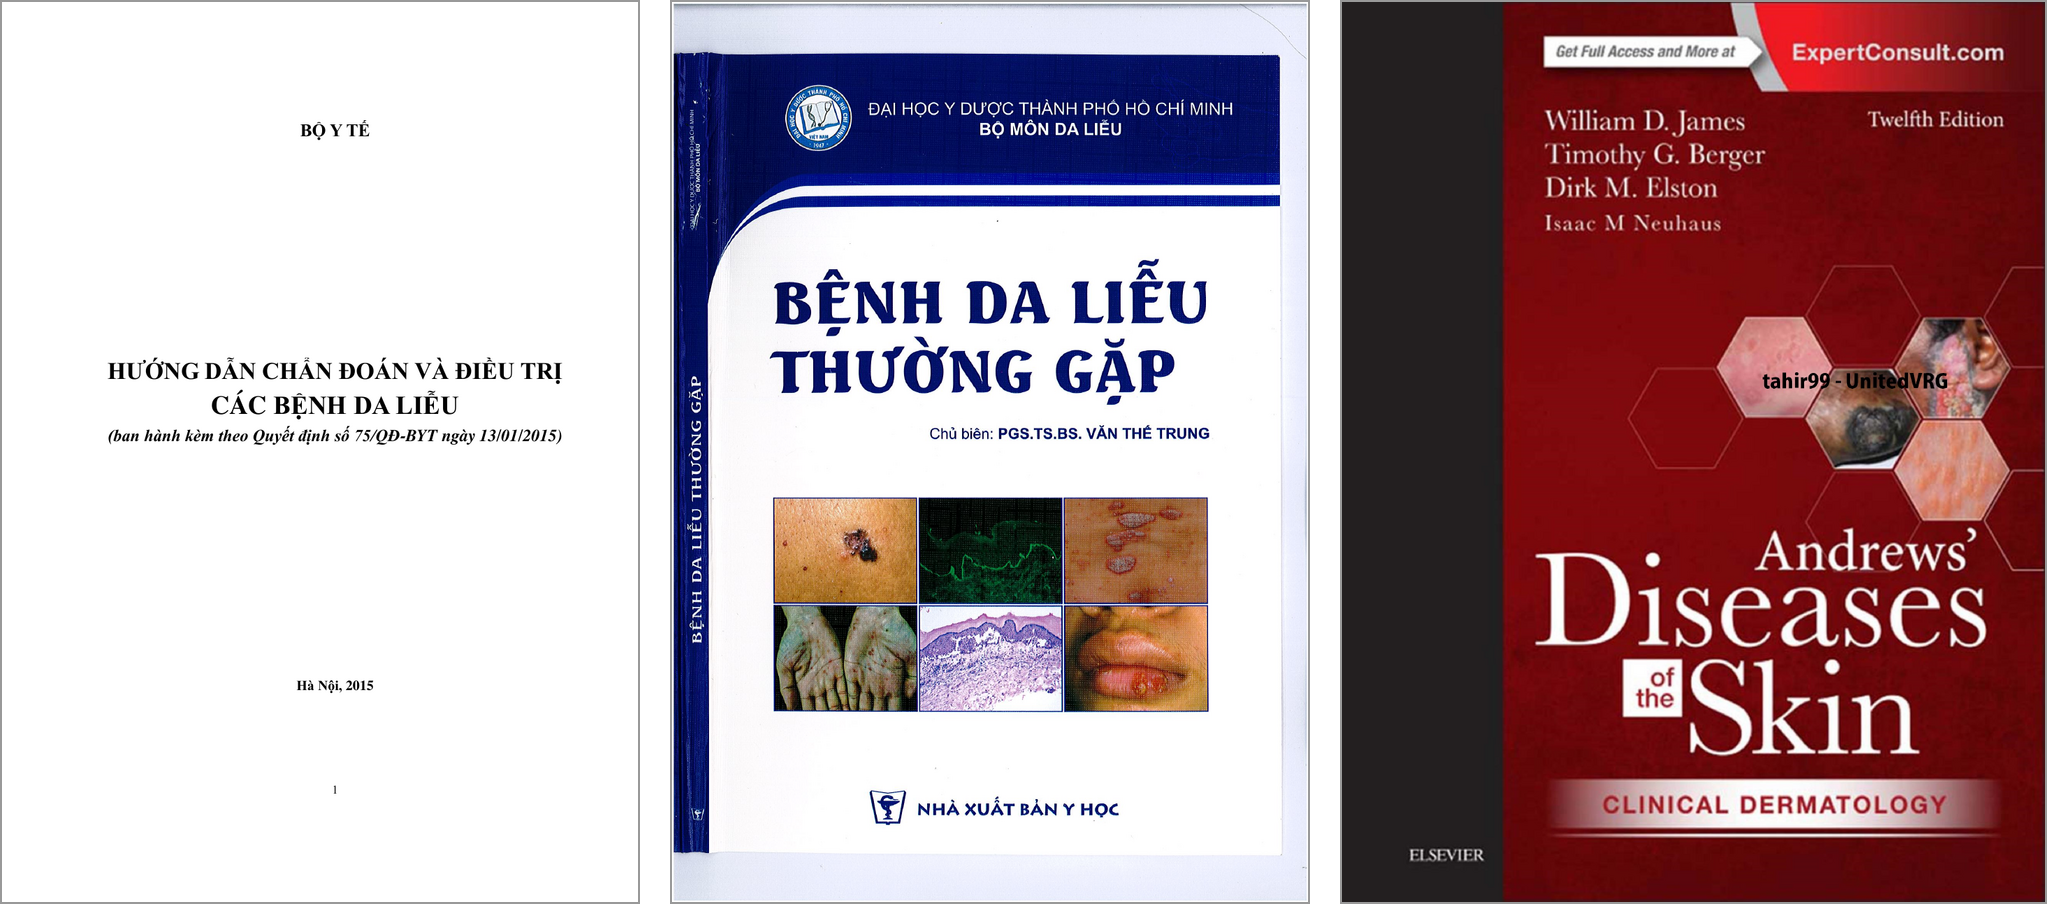
\includegraphics[width=\linewidth,height=0.45\textheight,keepaspectratio]{chuong4/hinh/bia-giao-trinh.png}
\caption{Ba giáo trình da liễu được số hóa}
\label{fig:bia-giao-trinh}
\end{figure}


\subsubsection{Quy trình số hóa giáo trình}

Quá trình số hóa gồm sáu bước, mỗi bước ghi kết quả rồi chờ người duyệt xác nhận. Một bước chỉ chạy khi các bước nó phụ thuộc đã được duyệt; ví dụ, chia đoạn chỉ chạy sau khi đã duyệt đọc nội dung và đọc mục lục.

\textbf{Bước 1. Đọc nội dung.} Docling nhận dạng chữ của PDF theo từng đoạn 20 trang và lưu kết quả sau mỗi đoạn, nên chạy lại không phải đọc lại. Mỗi trang cho ra chữ thân trang, số trang in và tiêu đề đầu trang; hình minh họa được lấy kèm.

\codeblock{chuong4/code/gt_doc_chu}{Mã đọc chữ theo từng đoạn trang bằng Docling}{lst:gt-doc-chu}

\textbf{Bước 2. Đọc mục lục.} LLM chuyển chữ các trang mục lục thành danh sách mục; mục có số trang đáng ngờ được đánh dấu để người duyệt kiểm tra. Hệ thống rồi ước lượng độ lệch giữa số trang in và số trang PDF, dựng cây mục và neo từng mục vào dòng tiêu đề trong thân sách.

\codeblock{chuong4/code/gt_muc_luc}{Mã đọc mục lục bằng LLM}{lst:gt-muc-luc}
\codeblock{chuong4/code/gt_do_lech}{Mã áp chỉnh sửa, tính độ lệch và neo mục}{lst:gt-do-lech}

\textbf{Bước 3. Chia đoạn.} Hệ thống tính lại độ lệch và neo mục theo chữ mới nhất, rồi chia chữ cho mục chứa nó và gom thành chunk dài tối đa 400 token ước lượng, không vượt ranh giới mục. Chunk bất thường (quá dài, quá ngắn, ranh giới chưa chính xác) được đưa vào danh sách cần soát.

\codeblock{chuong4/code/gt_chia_doan}{Mã chia đoạn theo khung mục lục}{lst:gt-chia-doan}

\textbf{Bước 4. Lưu vào kho tri thức.} Hệ thống tạo embedding cho từng chunk (kèm tên sách và đường dẫn mục) theo lô 64, rồi thay các point cũ của tài liệu bằng point mới trong Qdrant (point là bản ghi gồm vector dense, vector sparse BM25 và thông tin đi kèm). Số point lưu lệch số chunk thì bước báo lỗi.

\codeblock{chuong4/code/gt_luu_kho}{Mã tạo embedding cho chunk}{lst:gt-luu-kho}

\textbf{Bước 5. Trích quan hệ.} Bước này chạy song song với bước 4 và cùng dùng các chunk. Hệ thống chia chunk thành các lô gồm vài chunk liền nhau, mỗi lô không vượt ranh giới mục nhỏ nhất của mục lục. LLM đọc từng lô, điền quan hệ vào các ô của lược đồ và tự nêu chủ thể (bệnh hoặc thuốc) của mỗi quan hệ. Hệ thống chỉ giữ quan hệ có câu trích nằm nguyên văn trong chunk và khớp thực thể vào từ điển PrimeKG, DermO; người duyệt loại hoặc sửa trước khi nạp.

\codeblock{chuong4/code/dt_doc_trich}{Mã trích quan hệ từ chunk}{lst:dt-doc-trich}

\textbf{Bước 6. Lưu vào đồ thị tri thức.} Hệ thống lấy các quan hệ đã duyệt và khớp đủ hai đầu, dựng nút và cạnh (cạnh trùng cặp nút được gộp, nguồn ghi sách và số trang in), thay toàn bộ nút và cạnh của sách trong Neo4j rồi đếm lại; số cạnh lệch thì bước báo lỗi.

\codeblock{chuong4/code/dt_doc_nap}{Mã nạp quan hệ vào đồ thị}{lst:dt-doc-nap}

\subsubsection{Kết quả số hóa giáo trình}

\textbf{Kết quả trực quan.}

Hình~\ref{fig:pipeline-sach} là tổng quan quy trình số hóa; các hình tiếp theo là kết quả của từng bước.

\begin{figure}[H]
\centering
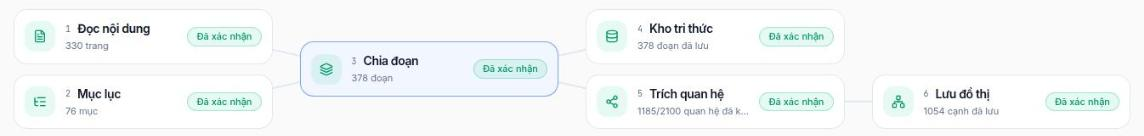
\includegraphics[width=0.95\linewidth,height=0.7\textheight,keepaspectratio]{chuong4/hinh/pipeline-tong-quan.png}
\caption{Tổng quan quy trình số hóa giáo trình}
\label{fig:pipeline-sach}
\end{figure}

\begin{figure}[H]
\centering
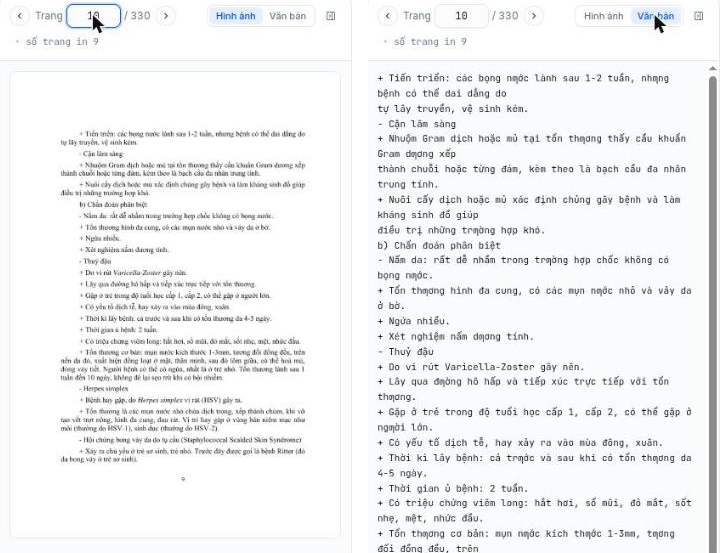
\includegraphics[width=0.8\linewidth,height=0.7\textheight,keepaspectratio]{chuong4/hinh/doc-noi-dung.png}
\caption{Kết quả đọc nội dung của một trang}
\label{fig:ket-qua-doc-noi-dung}
\end{figure}

\begin{figure}[H]
\centering
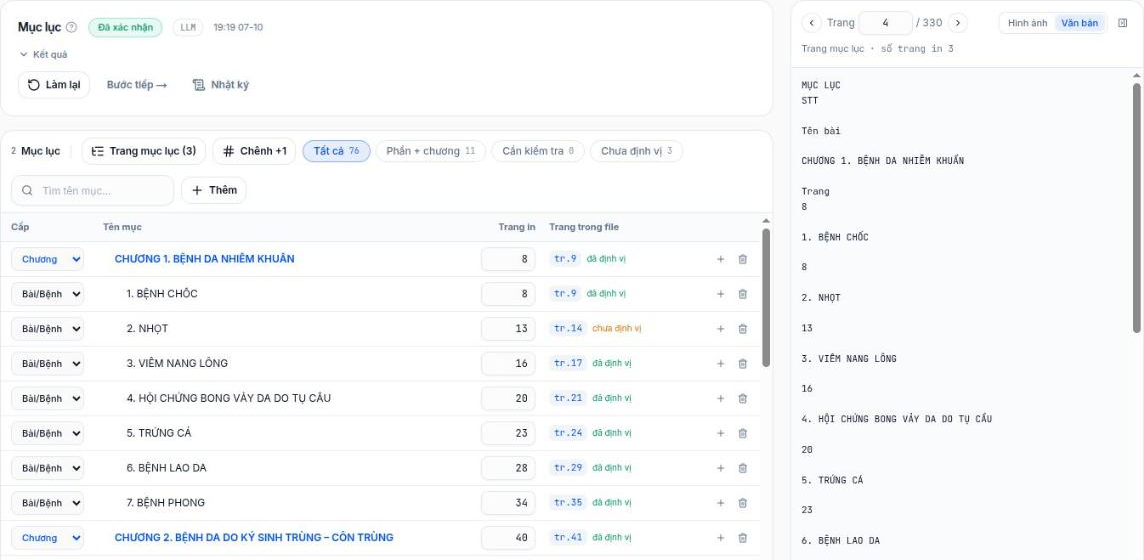
\includegraphics[width=0.95\linewidth,height=0.7\textheight,keepaspectratio]{chuong4/hinh/ket-qua-muc-luc.png}
\caption{Kết quả đọc mục lục của một sách}
\label{fig:ket-qua-muc-luc}
\end{figure}

\begin{figure}[H]
\centering
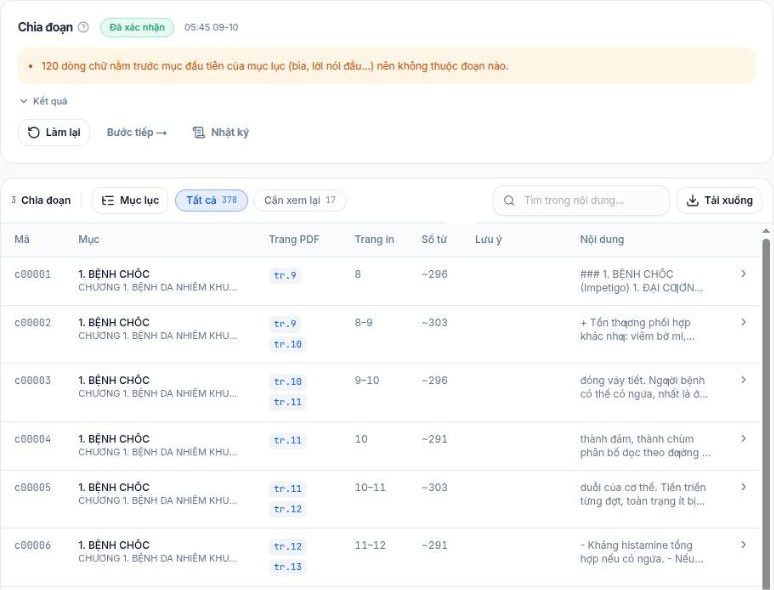
\includegraphics[width=0.9\linewidth,height=0.7\textheight,keepaspectratio]{chuong4/hinh/ket-qua-chia-doan.png}
\caption{Kết quả chia đoạn: chunk mẫu và danh sách cần soát}
\label{fig:ket-qua-chia-doan}
\end{figure}

\begin{figure}[H]
\centering
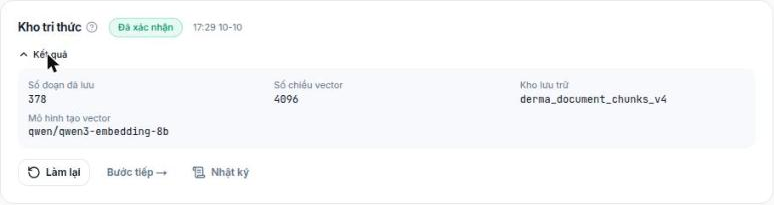
\includegraphics[width=0.9\linewidth,height=0.7\textheight,keepaspectratio]{chuong4/hinh/ket-qua-luu-kho.png}
\caption{Kết quả lưu vào kho tri thức: số đoạn đã lưu, số chiều vector, kho lưu trữ và mô hình tạo vector}
\label{fig:ket-qua-luu-kho}
\end{figure}

\begin{figure}[H]
\centering
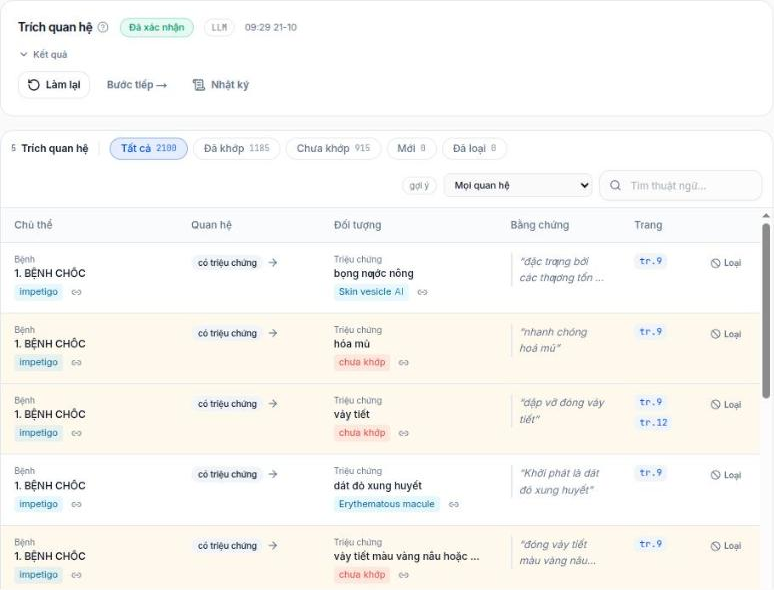
\includegraphics[width=0.9\linewidth,height=0.7\textheight,keepaspectratio]{chuong4/hinh/triple-browser.png}
\caption{Kết quả trích quan hệ: giao diện duyệt}
\label{fig:triple-browser}
\end{figure}

\textbf{Thông tin dữ liệu.}

Mỗi chunk là một point trong Qdrant, mang hai vector:
\begin{itemize}
  \item \textbf{Vector dense:} 4096 chiều, từ mô hình \texttt{qwen/qwen3-embedding-8b}, dùng cho tìm kiếm ngữ nghĩa.
  \item \textbf{Vector sparse:} tần suất từ theo BM25, dùng cho tìm kiếm từ khóa.
\end{itemize}

Thông tin đi kèm (payload) của point ghi \texttt{document\_id}, part, section, mục, số trang, mã các hình trong khoảng trang (\texttt{figure\_ids}) và đường dẫn file PDF gốc (\texttt{source\_pdf}).

\begin{table}[H]
\centering
\caption{Thống kê ba giáo trình đã nạp vào kho}
\label{tab:thong-ke-sach}
\small
\begin{tabular}{|p{5.2cm}|p{2.2cm}|p{1.6cm}|p{1.8cm}|p{2.4cm}|}
\hline
\textbf{Sách} & \textbf{Ngôn ngữ} & \textbf{Số trang} & \textbf{Số chunk} & \textbf{Số cạnh \texttt{DOC}} \\ \hline
Hướng dẫn chẩn đoán điều trị da liễu (Bộ Y tế) & Việt & 330 & 378 & 798 \\ \hline
Bệnh da liễu thường gặp (ĐH Y Dược TP.HCM) & Việt & 249 & 308 & 273 \\ \hline
Andrews' Diseases of the Skin & Anh & 1.083 & 4.232 & 7.731 \\ \hline
\end{tabular}
\end{table}

\begin{figure}[H]
\centering
\begin{tikzpicture}
\begin{axis}[
  xbar, width=0.8\linewidth, height=5cm, bar width=14pt,
  symbolic y coords={Andrews,{ĐH Y Dược TP.HCM},{Bộ Y tế}},
  ytick={Andrews,{ĐH Y Dược TP.HCM},{Bộ Y tế}}, y dir=reverse, enlarge y limits=0.3, xmin=0, xmax=5200,
  nodes near coords, nodes near coords align={horizontal},
  every node near coord/.append style={font=\small, text=black},
  /pgf/number format/.cd, fixed, set thousands separator={.}, precision=0,
  tick label style={font=\small}, xlabel={Số chunk}, xmajorgrids=true, grid style={gray!25},
  legend pos=south east, legend style={font=\small}, legend cell align=left]
\addplot[fill=blue!45!black!70, draw=none] coordinates {(308,{ĐH Y Dược TP.HCM}) (378,{Bộ Y tế})};
\addplot[fill=orange!70!black!75, draw=none] coordinates {(4232,Andrews)};
\legend{Tiếng Việt,Tiếng Anh}
\end{axis}
\end{tikzpicture}
\caption{Số chunk của ba giáo trình trong Qdrant}
\label{fig:chunk-theo-sach}
\end{figure}

Bước 6 đã nạp 8.802 cạnh từ ba sách (hình~\ref{fig:canh-doc-theo-sach}). Bước trích quan hệ cho ra 21.754 quan hệ, trong đó 10.267 quan hệ khớp đủ hai đầu vào PrimeKG hoặc DermO. Hệ thống bỏ 887 quan hệ có hai đầu trùng nút và gộp 578 quan hệ trùng cặp nút, còn 8.802 cạnh. Sách Fitzpatrick's Color Atlas mới qua bước chia đoạn (370 chunk), chưa lưu vào kho nên không nằm trong thống kê.

\begin{figure}[H]
\centering
\begin{tikzpicture}
\begin{axis}[
  xbar stacked, width=0.78\linewidth, height=7.6cm, bar width=9pt,
  symbolic y coords={DISEASE\_PHENOTYPE\_POSITIVE,INDICATION,ASSOCIATED\_WITH,IS\_A,DISEASE\_DISEASE,DISEASE\_PROTEIN,RESULTS\_IN,DISEASE\_PHENOTYPE\_NEGATIVE,DRUG\_EFFECT,EXPOSURE\_DISEASE,OFF\_LABEL\_USE,CONTRAINDICATION},
  ytick=data, y dir=reverse, enlarge y limits=0.06, xmin=0, xmax=4300,
  tick label style={font=\scriptsize}, xlabel={Số cạnh \texttt{DOC}}, xmajorgrids=true, grid style={gray!25},
  legend style={at={(0.97,0.5)}, anchor=east, font=\scriptsize}, legend cell align=left]
\addplot[fill=orange!70!black!75, draw=none] coordinates {(354,DISEASE\_PHENOTYPE\_POSITIVE) (198,INDICATION) (19,ASSOCIATED\_WITH) (78,IS\_A) (58,DISEASE\_DISEASE) (11,DISEASE\_PROTEIN) (18,RESULTS\_IN) (27,DISEASE\_PHENOTYPE\_NEGATIVE) (17,DRUG\_EFFECT) (11,EXPOSURE\_DISEASE) (1,OFF\_LABEL\_USE) (6,CONTRAINDICATION)};
\addplot[fill=teal!60!black!75, draw=none] coordinates {(93,DISEASE\_PHENOTYPE\_POSITIVE) (74,INDICATION) (15,ASSOCIATED\_WITH) (34,IS\_A) (23,DISEASE\_DISEASE) (10,DISEASE\_PROTEIN) (7,RESULTS\_IN) (4,DISEASE\_PHENOTYPE\_NEGATIVE) (10,DRUG\_EFFECT) (3,EXPOSURE\_DISEASE) (0,OFF\_LABEL\_USE) (0,CONTRAINDICATION)};
\addplot[fill=blue!45!black!70, draw=none] coordinates {(3565,DISEASE\_PHENOTYPE\_POSITIVE) (1415,INDICATION) (892,ASSOCIATED\_WITH) (530,IS\_A) (390,DISEASE\_DISEASE) (354,DISEASE\_PROTEIN) (226,RESULTS\_IN) (128,DISEASE\_PHENOTYPE\_NEGATIVE) (126,DRUG\_EFFECT) (74,EXPOSURE\_DISEASE) (24,OFF\_LABEL\_USE) (7,CONTRAINDICATION)};
\legend{Bộ Y tế,ĐH Y Dược TP.HCM,Andrews}
\end{axis}
\end{tikzpicture}
\caption{Số cạnh trích từ giáo trình theo loại quan hệ và theo sách (tổng 8.802 cạnh, ba sách)}
\label{fig:canh-doc-theo-sach}
\end{figure}

Hai loại quan hệ chiếm nhiều nhất là \texttt{DISEASE\_PHENOTYPE\_POSITIVE} (4.012 cạnh) và \texttt{INDICATION} (1.687 cạnh); hai loại này phục vụ các câu hỏi về triệu chứng và điều trị của bệnh.

\subsection{Ca bệnh đã kết luận của bác sĩ}

\subsubsection{Nội dung và vai trò của ca bệnh}

Ca bệnh đã kết luận là báo cáo kết luận do bác sĩ chốt khi đóng ca một phiên tư vấn. Mỗi phiên có một báo cáo và bác sĩ không sửa sau khi chốt. Chatbot dùng kho này để đối chiếu biểu hiện của người bệnh với các ca thực tế tương tự; kết quả chỉ để tham khảo, không phải chẩn đoán y khoa.

\subsubsection{Quy trình nạp ca bệnh vào Qdrant}

Hệ thống nạp ca vào một bộ lưu riêng trong Qdrant ngay sau khi bác sĩ lưu báo cáo kết luận.

\textbf{Bước 1. Tổng hợp văn bản.} Hệ thống đọc bản chụp (snapshot) của báo cáo lúc bác sĩ chốt và ghép thành một văn bản gồm chẩn đoán, thông tin bệnh nhân, dữ kiện lâm sàng, nhận định, dặn dò và thông tin ảnh, cùng thông tin đi kèm (payload), không chứa thông tin cá nhân (họ tên, số điện thoại).

\codeblock{chuong4/code/cb_van_ban}{Mã tổng hợp văn bản và payload của ca bệnh}{lst:cb-van-ban}

\textbf{Bước 2. Tạo vector và nạp point.} Hệ thống tính embedding dense và vector sparse BM25 (chế độ hỗn hợp Việt -- Anh) từ cùng văn bản, rồi ghi một point vào Qdrant.

\codeblock{chuong4/code/cb_nap_point}{Mã nạp một ca bệnh vào Qdrant}{lst:cb-nap-point}

\subsubsection{Kết quả nạp ca bệnh}

\textbf{Kết quả trực quan.}

\begin{figure}[H]
\centering
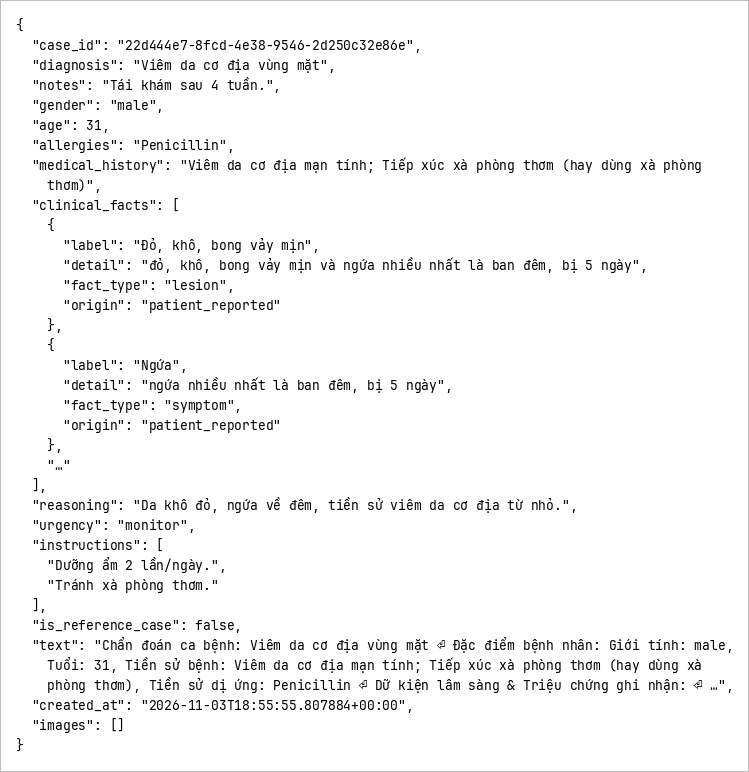
\includegraphics[width=0.75\linewidth,height=0.7\textheight,keepaspectratio]{chuong4/hinh/ca-benh-point.png}
\caption{Thông tin đi kèm của một ca bệnh trong Qdrant}
\label{fig:ca-benh-point}
\end{figure}

\textbf{Thông tin dữ liệu.} Mọi báo cáo đã chốt đều được nạp, kể cả ca chưa đánh dấu là ca tham khảo; dấu này hiện chỉ được ghi kèm, chưa dùng để lọc khi tra. Bảng~\ref{tab:cb-payload} liệt kê thông tin đi kèm mỗi point.

\begin{table}[H]
\centering
\caption{Thông tin đi kèm mỗi ca bệnh trong Qdrant}
\label{tab:cb-payload}
\small
\begin{tabular}{|p{4.0cm}|p{9.5cm}|}
\hline
\textbf{Trường} & \textbf{Ý nghĩa} \\ \hline
\texttt{case\_id} & Mã ca; mã point được sinh từ mã này \\ \hline
\texttt{diagnosis} & Chẩn đoán do bác sĩ chốt \\ \hline
\texttt{is\_reference\_case} & Dấu ca tham khảo do bác sĩ đặt \\ \hline
\texttt{created\_at} & Thời điểm tạo báo cáo \\ \hline
\texttt{gender} & Giới tính \\ \hline
\texttt{age} & Tuổi, tính từ năm sinh \\ \hline
\texttt{allergies} & Dị ứng \\ \hline
\texttt{medical\_history} & Tiền sử bệnh \\ \hline
\texttt{clinical\_facts} & Dữ kiện lâm sàng ghi nhận trong phiên \\ \hline
\texttt{reasoning} & Nhận định của bác sĩ \\ \hline
\texttt{urgency} & Mức khẩn cấp \\ \hline
\texttt{instructions} & Dặn dò và hướng xử trí \\ \hline
\texttt{notes} & Ghi chú bổ sung \\ \hline
\texttt{text} & Văn bản dùng để tạo vector \\ \hline
\texttt{images} & Ảnh gắn vào ca: nhãn đã xác nhận, vị trí, mô tả, tên và đường dẫn file \\ \hline
\end{tabular}
\end{table}

Hiện có 14 ca bệnh đã kết luận trong kho.

\subsection{Đồ thị tri thức có sẵn: PrimeKG và DermO}
\label{sec:do-thi-tri-thuc}

\subsubsection{Nội dung và vai trò của đồ thị}

Neo4j chứa đồ thị có sẵn gồm hai phần, cùng quan hệ trích từ giáo trình (mục~\ref{sec:giao-trinh}):
\begin{itemize}
  \item \textbf{PrimeKG:} đồ thị y sinh có sẵn. Hệ thống giữ 5 loại nút (bệnh, thuốc, phenotype, gen/protein, phơi nhiễm) và 11 loại quan hệ, khoảng 3,46 triệu cạnh.
  \item \textbf{DermO:} ontology da liễu, 3.427 thuật ngữ, mỗi thuật ngữ có từ đồng nghĩa và thuật ngữ cha. Dùng để chuẩn hóa tên, không dùng để suy ra quan hệ lâm sàng.
\end{itemize}

PrimeKG và DermO không có cạnh nối nhau; hệ thống nối chúng bằng so khớp tên lúc truy vấn.

\begin{figure}[H]
\centering
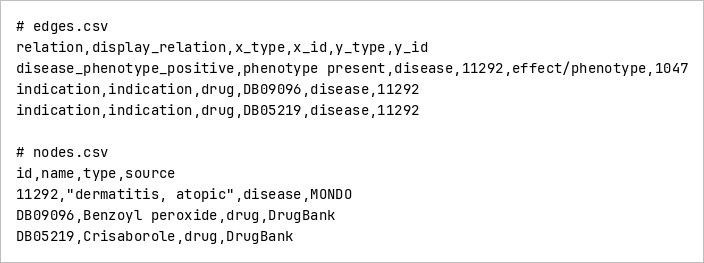
\includegraphics[width=0.85\linewidth,height=0.7\textheight,keepaspectratio]{chuong4/hinh/nguon-primekg.png}
\caption{Dữ liệu PrimeKG sau khi lọc: bảng cạnh và bảng nút}
\label{fig:nguon-primekg}
\end{figure}

\begin{figure}[H]
\centering
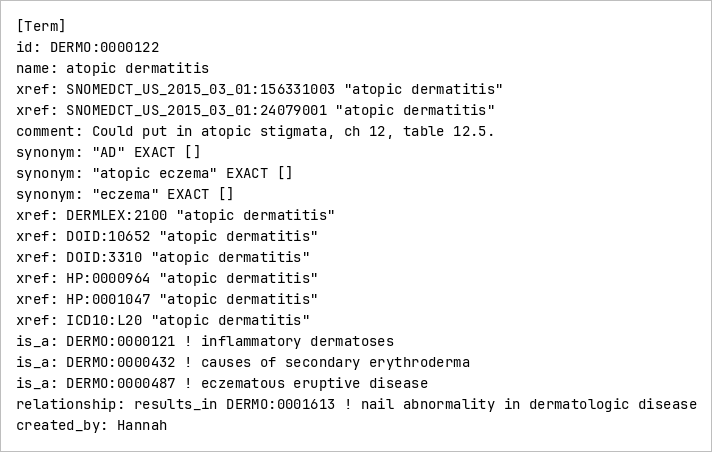
\includegraphics[width=0.85\linewidth,height=0.7\textheight,keepaspectratio]{chuong4/hinh/nguon-dermo.png}
\caption{Dữ liệu nguồn của DermO: một khối thuật ngữ}
\label{fig:nguon-dermo}
\end{figure}

\subsubsection{Quy trình nạp đồ thị vào Neo4j}

Hai phần có sẵn được dựng như sau.

\textbf{PrimeKG, bước 1. Lọc.} Nguồn là bảng quan hệ của PrimeKG (Harvard Dataverse, phiên bản 2). Hệ thống chỉ giữ 5 loại nút và 11 loại quan hệ trong phạm vi, bỏ dòng thiếu mã và cạnh trùng, rồi ghi danh sách nút và cạnh trung gian.

\codeblock{chuong4/code/dt_primekg_loc}{Mã lọc quan hệ PrimeKG}{lst:dt-primekg-loc}

\textbf{PrimeKG, bước 2. Nạp vào Neo4j.} Hệ thống nạp cạnh theo lô; quan hệ đã có cạnh được gộp (merge) để nạp lại không nhân đôi.

\codeblock{chuong4/code/dt_primekg_nap}{Mã nạp cạnh PrimeKG}{lst:dt-primekg-nap}

\textbf{DermO, bước 1. Đọc tệp ontology.} Tệp DermO (định dạng OBO, phiên bản 1.19) gồm các khối thuật ngữ; hệ thống đọc mỗi khối thành một thuật ngữ có tên, định nghĩa, từ đồng nghĩa, thuật ngữ cha và các quan hệ.

\codeblock{chuong4/code/dt_dermo_doc}{Mã đọc tệp ontology DermO}{lst:dt-dermo-doc}

\textbf{DermO, bước 2. Nạp vào Neo4j.} Mỗi thuật ngữ thành một nút \texttt{DermoTerm}. Quan hệ ``là một'' (\texttt{is\_a}) thành cạnh \texttt{IS\_A}; các quan hệ khác giữ tên gốc viết hoa (ví dụ \texttt{HAS\_SYMPTOM}, \texttt{RESULTS\_IN}).

\codeblock{chuong4/code/dt_dermo_nap}{Mã nạp cạnh DermO}{lst:dt-dermo-nap}

\subsubsection{Kết quả nạp đồ thị}

\textbf{Kết quả trực quan.}

Hình~\ref{fig:schema-neo4j} là lược đồ (schema) của đồ thị tri thức, lấy từ Neo4j Browser bằng \texttt{db.schema.visualization()}, gồm năm loại nút của PrimeKG và nút \texttt{DermoTerm} của DermO. Hình đã lọc bỏ các nhãn của đồ thị hành trình bệnh nhân. Mỗi vòng tự nối là một loại quan hệ giữa hai nút cùng loại; các quan hệ nối \texttt{DermoTerm} (\texttt{IS\_A}, \texttt{HAS\_SYMPTOM}, \ldots) gồm cả cạnh trích từ giáo trình.

\begin{figure}[H]
\centering
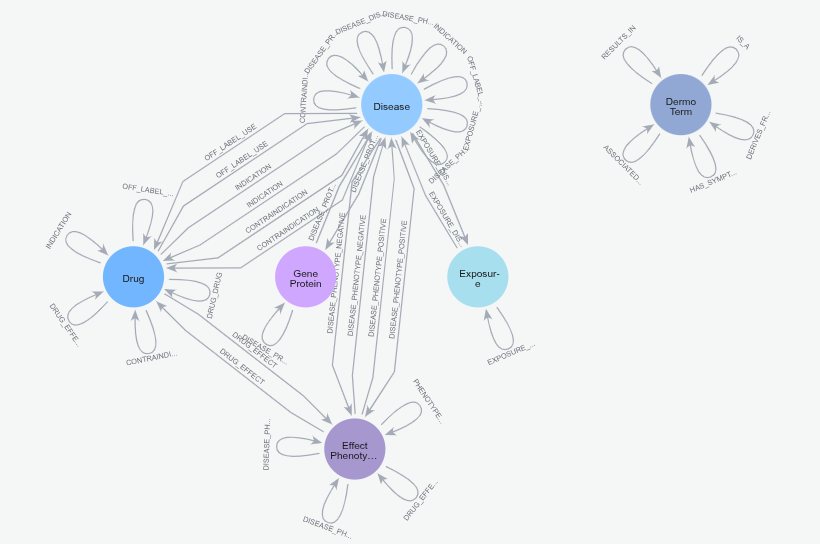
\includegraphics[width=0.95\linewidth,height=0.6\textheight,keepaspectratio]{chuong4/hinh/schema-neo4j.png}
\caption{Lược đồ đồ thị tri thức trong Neo4j Browser (sáu loại nút, không gồm đồ thị hành trình bệnh nhân)}
\label{fig:schema-neo4j}
\end{figure}

\begin{figure}[H]
\centering
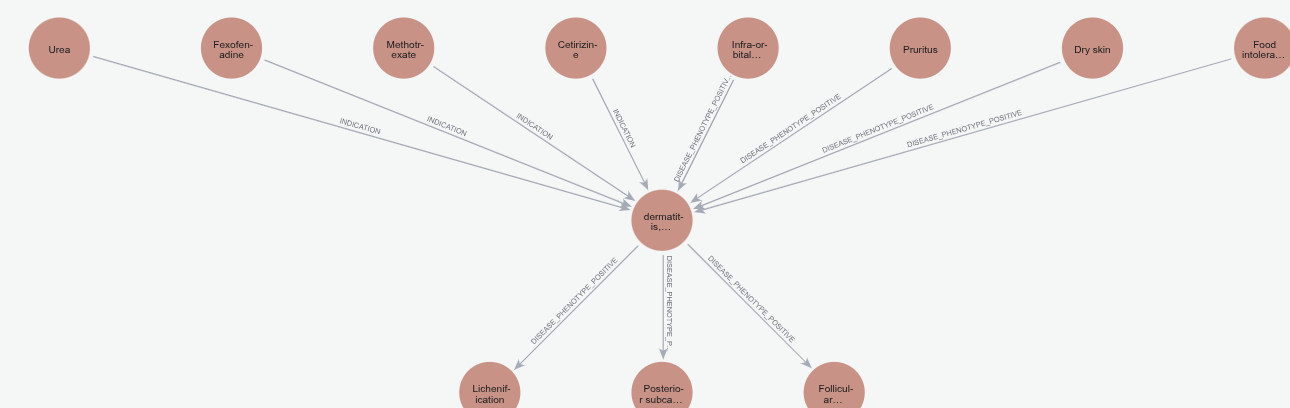
\includegraphics[width=\linewidth,keepaspectratio]{chuong4/hinh/do-thi-mau.png}
\caption{Đồ thị quanh bệnh \textit{dermatitis, atopic} trong Neo4j Browser: thuốc chỉ định (cạnh \texttt{INDICATION}) và triệu chứng, dấu hiệu lâm sàng của bệnh (cạnh \texttt{DISEASE\_PHENOTYPE\_POSITIVE})}
\label{fig:do-thi-mau}
\end{figure}

\begin{figure}[H]
\centering
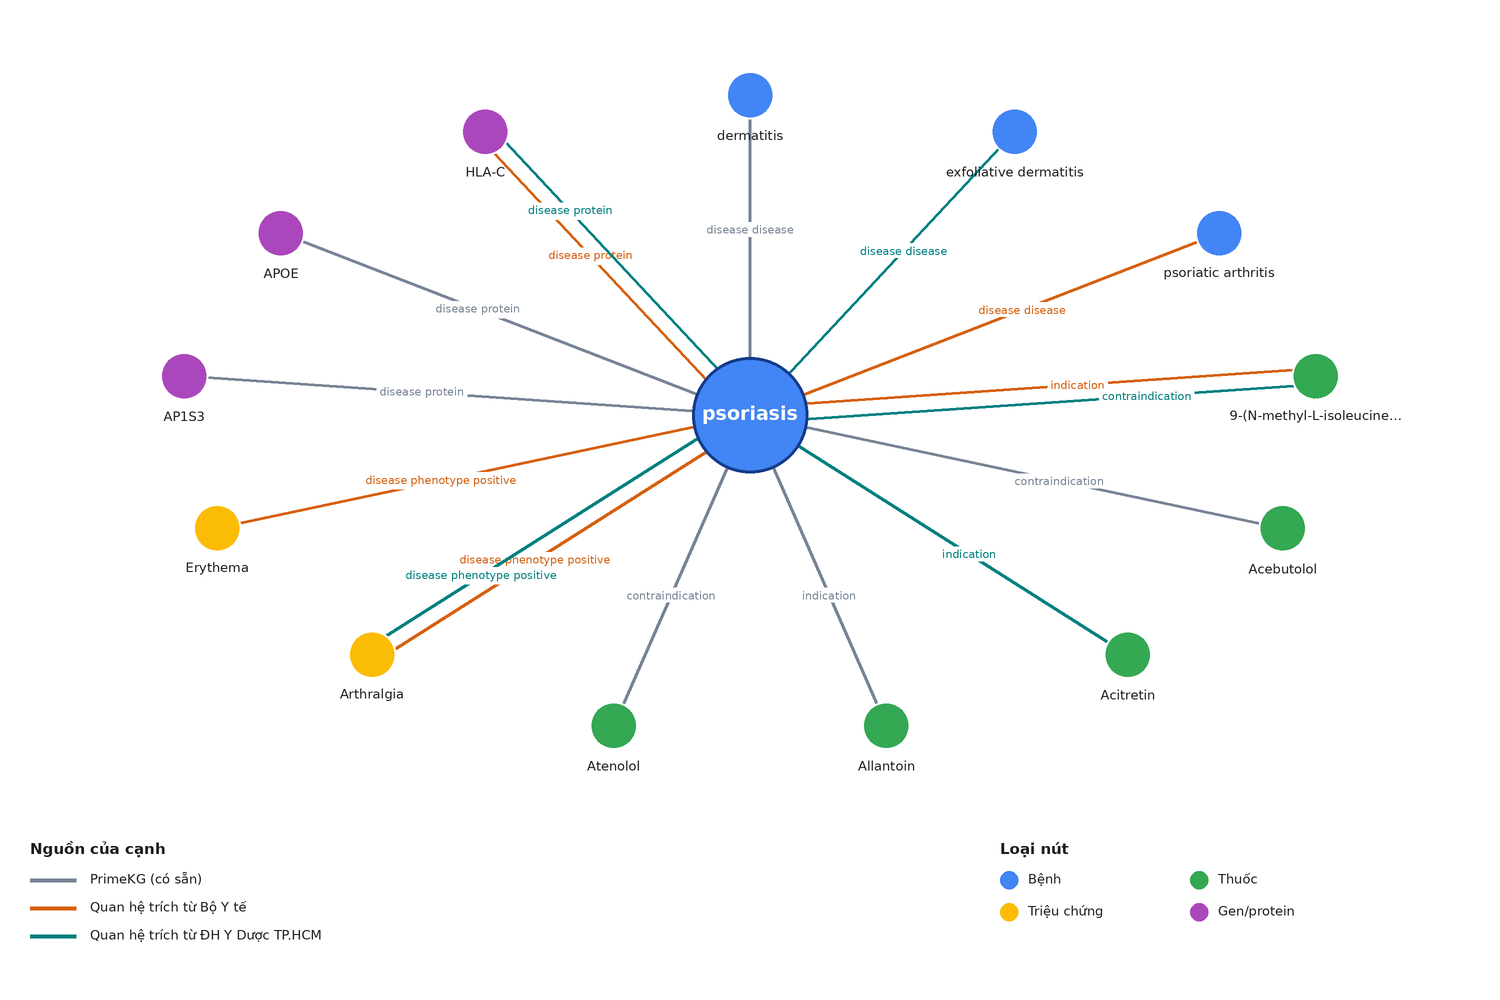
\includegraphics[width=0.95\linewidth,height=0.7\textheight,keepaspectratio]{chuong4/hinh/so-sanh-nguon-canh.png}
\caption{Cạnh PrimeKG và cạnh trích từ hai giáo trình quanh bệnh psoriasis}
\label{fig:so-sanh-nguon-canh}
\end{figure}


\textbf{Thông tin dữ liệu.}

Hình~\ref{fig:primekg-nut} và~\ref{fig:primekg-canh} thống kê PrimeKG đã nạp. Loại cạnh \texttt{DRUG\_DRUG} chiếm khoảng 77\% tổng số cạnh nên trục số cạnh dùng thang logarit. Các truy vấn của chatbot không duyệt loại cạnh này.

\begin{figure}[H]
\centering
\begin{tikzpicture}
\begin{axis}[
  xbar, width=0.85\linewidth, height=5.2cm, bar width=12pt,
  symbolic y coords={Phơi nhiễm,Thuốc,Gen/protein,Phenotype,Bệnh}, ytick=data,
  xmin=0, xmax=21000, enlarge y limits=0.15, scaled x ticks=false, xtick={0,5000,10000,15000,20000},
  nodes near coords, nodes near coords align={horizontal},
  every node near coord/.append style={font=\small, text=black},
  /pgf/number format/.cd, fixed, set thousands separator={.}, precision=0,
  xlabel={Số nút}, tick label style={font=\small}, xmajorgrids=true, grid style={gray!25},
  ]
\addplot[fill=blue!45!black!70, draw=none] coordinates {(474,Phơi nhiễm) (4540,Thuốc) (9080,Gen/protein) (15310,Phenotype) (17080,Bệnh)};
\end{axis}
\end{tikzpicture}
\caption{Số nút của PrimeKG theo loại (bệnh gồm cả nhóm \texttt{MONDO\_grouped})}
\label{fig:primekg-nut}
\end{figure}

\begin{figure}[H]
\centering
\begin{tikzpicture}
\begin{axis}[
  xbar, width=0.78\linewidth, height=8.6cm, bar width=9pt, xmode=log, log origin=infty,
  xmin=1000, xmax=60000000,
  symbolic y coords={DISEASE\_PHENOTYPE\_NEGATIVE,EXPOSURE\_DISEASE,OFF\_LABEL\_USE,INDICATION,PHENOTYPE\_PHENOTYPE,CONTRAINDICATION,DISEASE\_DISEASE,DRUG\_EFFECT,DISEASE\_PROTEIN,DISEASE\_PHENOTYPE\_POSITIVE,DRUG\_DRUG},
  ytick=data, y dir=reverse, enlarge y limits=0.06,
  nodes near coords,
  every node near coord/.append style={font=\scriptsize, text=black, anchor=west, xshift=2pt, yshift=0pt}, point meta=explicit symbolic,
  /pgf/number format/.cd, fixed, set thousands separator={.}, precision=0,
  xlabel={Số cạnh (thang logarit)}, tick label style={font=\scriptsize}, xmajorgrids=true, grid style={gray!25},
  ]
\addplot[fill=teal!60!black!75, draw=none] coordinates {(2672628,DRUG\_DRUG) [2.672.628] (300634,DISEASE\_PHENOTYPE\_POSITIVE) [300.634] (160822,DISEASE\_PROTEIN) [160.822] (129568,DRUG\_EFFECT) [129.568] (64388,DISEASE\_DISEASE) [64.388] (61350,CONTRAINDICATION) [61.350] (37472,PHENOTYPE\_PHENOTYPE) [37.472] (18776,INDICATION) [18.776] (5136,OFF\_LABEL\_USE) [5.136] (4608,EXPOSURE\_DISEASE) [4.608] (2386,DISEASE\_PHENOTYPE\_NEGATIVE) [2.386]};
\end{axis}
\end{tikzpicture}
\caption{Số cạnh của PrimeKG theo loại quan hệ}
\label{fig:primekg-canh}
\end{figure}


\section{Các luồng truy xuất tri thức của chatbot}
\label{sec:luong-truy-xuat}

\subsection{Truy xuất trong luồng RAG của chatbot}
\label{sec:rag-tong-quan}

Truy xuất tăng cường sinh văn bản (RAG) gồm hai phần: tìm bằng chứng trong kho tri thức, rồi để mô hình ngôn ngữ sinh câu trả lời dựa trên bằng chứng đó. Chatbot thực hiện bốn bước:
\begin{enumerate}
  \item \textbf{Nạp tri thức:} giáo trình được cắt thành đoạn và nạp vào Qdrant; quan hệ trích từ sách nạp vào Neo4j; ca bệnh nạp vào kho riêng (mục~\ref{sec:nguon-kb}).
  \item \textbf{Truy xuất:} agent gọi công cụ tra cứu, công cụ chạy ba hướng tìm kiếm ngữ nghĩa, từ khóa, đồ thị và gộp kết quả bằng RRF (các mục từ~\ref{sec:luong-ngu-nghia} đến~\ref{sec:luong-hon-hop}).
  \item \textbf{Đưa bằng chứng vào ngữ cảnh:} mỗi kết quả nhận một mã \texttt{E\#} kèm sách, mục và số trang (Chương~\ref{ch:chuong5}).
  \item \textbf{Sinh câu trả lời:} agent chỉ giữ giả thuyết có ít nhất một mã \texttt{E\#} hợp lệ; câu trả lời là gợi ý hỗ trợ, không phải chẩn đoán y khoa (Chương~\ref{ch:chuong5}).
\end{enumerate}
Chương này mô tả hai bước đầu. Hai bước sau thuộc luồng lập luận của agent ở Chương~\ref{ch:chuong5}.

\subsection{Các luồng truy xuất trên văn bản giáo trình}

Trên các đoạn giáo trình (chunk), hệ thống có ba hướng tìm kiếm. Hai hướng đầu, ngữ nghĩa và từ khóa, bổ sung cho nhau. Hướng thứ ba đi qua đồ thị: từ thực thể trong câu hỏi tới quan hệ đã trích từ sách, rồi tới các đoạn chứa câu trích của quan hệ đó (bảng~\ref{tab:bu-dap}). Ca bệnh đã kết luận dùng hai hướng đầu trên kho riêng; hướng đồ thị chỉ áp dụng cho giáo trình.

\begin{table}[H]
\centering
\caption{Ba hướng tìm kiếm bổ sung cho nhau}
\label{tab:bu-dap}
\small
\begin{tabular}{|p{2.0cm}|p{3.8cm}|p{3.8cm}|p{3.9cm}|}
\hline
\textbf{Tiêu chí} & \textbf{Ngữ nghĩa (dense)} & \textbf{Từ khóa (BM25, sparse)} & \textbf{Đồ thị (liên kết tới đoạn)} \\ \hline
So khớp & Cosine giữa vector câu hỏi và vector đoạn & Từ trùng, có trọng số theo độ hiếm & Tên thực thể trùng tên hoặc từ đồng nghĩa của nút; lấy đoạn gắn với quan hệ của nút \\ \hline
Bắt được & Diễn đạt khác nghĩa cùng; câu hỏi tiếng Việt, sách tiếng Anh & Tên thuốc, hoạt chất, mã bệnh, liều & Đoạn mà sách đã trích thành quan hệ với thực thể được hỏi, kể cả khi đoạn dùng từ khác \\ \hline
Bỏ sót & Token hiếm bị làm mờ trong vector & Câu hỏi và đoạn không có từ chung & Thực thể chưa có quan hệ trích từ sách; không đi qua nút lân cận \\ \hline
\end{tabular}
\end{table}

Ví dụ: câu hỏi ``da tôi đỏ và ngứa, nổi thành mảng'' và đoạn chứa ``erythematous pruritic plaques'' không có từ chung. BM25 cho điểm $0$, tìm kiếm ngữ nghĩa vẫn khớp. Ngược lại, câu hỏi về một tên thuốc cụ thể được BM25 khớp đúng chữ, trong khi vector có thể gộp thuốc đó với các thuốc cùng nhóm.


Mã nguồn đặc trưng của từng luồng được trích ở các mã nguồn~\ref{lst:ngu-nghia}, \ref{lst:bm25}, \ref{lst:graph-leg}, \ref{lst:rrf}, \ref{lst:hybrid} và~\ref{lst:seed}. Phần sau mô tả từng luồng đơn (mục~\ref{sec:luong-ngu-nghia}, \ref{sec:luong-tu-khoa} và~\ref{sec:luong-do-thi}), rồi luồng hỗn hợp ghép ba luồng đó (mục~\ref{sec:luong-hon-hop}).

\subsection{Luồng tìm kiếm ngữ nghĩa}
\label{sec:luong-ngu-nghia}

\subsubsection{Nguyên lý tìm kiếm ngữ nghĩa}

Tìm kiếm ngữ nghĩa so khớp theo nghĩa của câu thay vì theo ký tự. Mô hình embedding đổi mỗi đoạn văn bản thành một vector thực $d$ chiều. Bài toán tra cứu trở thành bài toán hình học: tìm các vector đoạn gần vector câu hỏi nhất.

Hệ thống dùng mô hình \texttt{qwen/qwen3-embedding-8b} (8 tỷ tham số), đầu ra $d=4096$ chiều. Mô hình có hai đặc tính:
\begin{itemize}
  \item \textbf{Instruction-tuned:} câu hỏi được thêm tiền tố chỉ dẫn; đoạn trong kho tri thức được mã hóa ở dạng nguyên bản.
  \item \textbf{Đa ngôn ngữ:} câu hỏi tiếng Việt và đoạn tiếng Anh nằm chung một không gian vector.
\end{itemize}

\subsubsection{Cơ chế tìm kiếm ngữ nghĩa}

Gọi $f$ là hàm embedding. Quy trình có hai giai đoạn:
\begin{itemize}
  \item \textbf{Nạp dữ liệu (indexing):} mỗi đoạn được mã hóa một lần, $d=f(\text{đoạn})$, rồi lưu vào Qdrant.
  \item \textbf{Truy vấn (querying):} câu hỏi được mã hóa một lần, $q=f(\text{câu hỏi})$. Kiến trúc Bi-Encoder mã hóa câu hỏi và đoạn độc lập, nên vector đoạn được tính trước và độ trễ lúc truy vấn thấp.
\end{itemize}

Độ liên quan giữa $q$ và $d$ là độ tương đồng cosine:
\begin{equation}
  \mathrm{sim}(q,d)=\frac{q\cdot d}{\Vert q\Vert \Vert d\Vert }
\end{equation}

Trong đó, $\mathrm{sim}(q,d)\in[-1,1]$. Phép đo chỉ phụ thuộc hướng vector nên không bị lệch bởi độ dài đoạn.

Hệ thống xếp các đoạn theo $\mathrm{sim}$ giảm dần, lấy $k$ đoạn đầu, đọc nội dung và siêu dữ liệu (sách, mục, trang) theo ID vector rồi trả về.

\codeblock{chuong4/code/dense}{Mã tìm kiếm ngữ nghĩa: mã hóa câu hỏi (có tiền tố chỉ dẫn) và truy vấn Qdrant}{lst:ngu-nghia}

\subsection{Luồng tìm kiếm từ khóa}
\label{sec:luong-tu-khoa}

\subsubsection{Nguyên lý tìm kiếm từ khóa}

Tìm kiếm từ khóa khớp chính xác chuỗi ký tự. Luồng này bù cho điểm yếu của vector: tên thuốc, hoạt chất, mã bệnh và liều lượng thường bị làm mờ trong embedding.

\textbf{TF-IDF} là nền tảng của phương pháp. Điểm của tài liệu $D$ với câu hỏi $Q$ là tổng, trên các từ $t\in Q$, của tích tần suất từ trong tài liệu ($\mathrm{tf}$) và độ hiếm của từ trong kho ($\mathrm{idf}$):
\begin{equation}
  \mathrm{score}_{\mathrm{TF\text{-}IDF}}(D,Q)=\sum _{t\in Q} \mathrm{tf}(t,D)\cdot \mathrm{idf}(t)
\end{equation}
Hai thành phần được tính như sau:
\begin{equation}
  \mathrm{tf}(t,D)=f(t,D)
\end{equation}
\begin{equation}
  \mathrm{idf}(t)=\ln\frac{N}{n(t)}
\end{equation}
Trong đó $f(t,D)$ là số lần từ $t$ xuất hiện trong đoạn $D$, $N$ là tổng số đoạn trong kho và $n(t)$ là số đoạn chứa $t$. Từ xuất hiện trong ít đoạn có $\mathrm{idf}$ lớn nên đóng góp nhiều vào điểm. Từ có mặt ở mọi đoạn ($n(t)=N$) có $\mathrm{idf}=0$ và không ảnh hưởng đến điểm.

TF-IDF có hai hạn chế:
\begin{itemize}
  \item \textbf{Không bão hòa:} điểm tăng tuyến tính theo tần suất từ, dù từ lặp lại nhiều lần không làm đoạn liên quan hơn tương ứng.
  \item \textbf{Không chuẩn hóa độ dài:} đoạn dài chứa nhiều từ hơn nên được điểm cao hơn.
\end{itemize}

\subsubsection{Thuật toán xếp hạng BM25}

BM25 (Best Matching 25) thêm hai tham số để sửa hai hạn chế trên:
\begin{equation}
  \mathrm{score}(D,Q)=\sum_{t\in Q}\mathrm{IDF}(t)\cdot\frac{\mathrm{tf}\cdot(k_1+1)}{\mathrm{tf}+k_1\cdot\left(1-b+b\cdot\frac{|D|}{\mathrm{avgdl}}\right)}
\end{equation}
\begin{equation}
  \mathrm{IDF}(t)=\ln\left( 1+\frac{N-n(t)+0{,}5}{n(t)+0{,}5}\right)
\end{equation}

Trong đó:
\begin{itemize}
  \item $\mathrm{tf}(t,D)$: số lần từ $t$ xuất hiện trong $D$; $n(t)$: số đoạn chứa $t$; $N$: tổng số đoạn.
  \item $k_1=1{,}2$: giới hạn mức tăng điểm theo tần suất từ (độ bão hòa).
  \item $b=0{,}75$: mức chuẩn hóa theo tỷ số giữa độ dài đoạn $|D|$ và độ dài trung bình $\mathrm{avgdl}$.
\end{itemize}

Qdrant lưu phần $\mathrm{tf}$ của mỗi đoạn dưới dạng vector thưa (sparse) và chấm điểm khi truy vấn. Cấu trúc này hoạt động như chỉ mục đảo: mỗi từ trỏ tới các đoạn chứa nó, nên truy vấn không phải duyệt toàn bộ kho.

\subsubsection{Cơ chế tìm kiếm từ khóa}

\begin{itemize}
  \item \textbf{Mở rộng câu hỏi Việt -- Anh:} LLM trích thực thể y khoa từ câu hỏi và thêm tên tiếng Anh, tiếng Việt vào câu hỏi BM25, để khớp với sách viết khác ngôn ngữ câu hỏi. Khi LLM lỗi, BM25 dùng câu hỏi gốc và hệ thống ghi chú lại.
  \item \textbf{Tiền xử lý tiếng Việt:} tách từ ghép bằng underthesea, loại stopword nhưng giữ từ phủ định và đơn vị liều. Thêm token bỏ dấu với trọng số thấp ($0{,}3$) để câu hỏi không dấu vẫn khớp.
  \item \textbf{Cách dùng:} chạy độc lập khi cần tra tên chính xác, và là một nhánh của luồng hỗn hợp.
\end{itemize}

\codeblock{chuong4/code/sparse}{Mã chuyển văn bản thành vector thưa BM25: \texttt{encode\_document} lưu vào Qdrant, \texttt{encode\_query} dùng khi truy vấn}{lst:bm25}

\subsection{Luồng tìm kiếm đồ thị}
\label{sec:luong-do-thi}

\subsubsection{Nguyên lý tìm kiếm đồ thị}

Hai luồng trước so khớp câu hỏi với nội dung đoạn. Luồng đồ thị so khớp theo thực thể y khoa và đi ngược từ thực thể về đoạn. Quan hệ trích từ sách (mục~\ref{sec:giao-trinh}) lưu mã các đoạn chứa câu trích, nên từ một thực thể có thể lấy lại các đoạn đó, kể cả khi đoạn dùng từ khác với câu hỏi.

Điểm của đoạn $c$ là số quan hệ trỏ tới nó:
\begin{equation}
  \mathrm{score}_{G}(c)=\bigl|\{\,r\in R(E)\;:\;c\in \mathrm{chunks}(r)\,\}\bigr|
\end{equation}

Trong đó $E$ là tập nút đồ thị khớp với thực thể trong câu hỏi, $R(E)$ là tập quan hệ trích từ sách nối trực tiếp với một nút thuộc $E$, và $\mathrm{chunks}(r)$ là tập đoạn chứa câu trích của quan hệ $r$. Đoạn cùng điểm được xếp theo mã đoạn.

Luồng này trả về đoạn giáo trình. Việc truy vấn đồ thị để chọn bệnh ứng viên là chức năng khác, trình bày ở mục~\ref{sec:truy-xuat-do-thi}.

\subsubsection{Cơ chế tìm kiếm đồ thị}

Luồng chỉ chạy với kho giáo trình; với kho ca bệnh, luồng trả danh sách rỗng.
\begin{enumerate}
  \item \textbf{Lấy tên thực thể:} tên tiếng Anh và tiếng Việt của các thực thể y khoa trong câu hỏi, bỏ loại khác.
  \item \textbf{Tìm nút:} tối đa 10 nút của đồ thị có tên hoặc từ đồng nghĩa khớp, không phân biệt hoa thường. Hệ thống khớp chính xác trước, chỉ khi không có kết quả mới khớp theo chuỗi con.
  \item \textbf{Lấy đoạn từ quan hệ:} các quan hệ trích từ sách nối trực tiếp với những nút đó (một bước, không phân biệt hướng); mỗi quan hệ cho các đoạn chứa câu trích của nó.
  \item \textbf{Xếp hạng và lấy đoạn:} đoạn có nhiều quan hệ trỏ tới xếp trước, rồi lấy nội dung đoạn từ Qdrant.
\end{enumerate}

\codeblock{chuong4/code/graph_leg}{Mã luồng đồ thị: từ thực thể tới đoạn giáo trình}{lst:graph-leg}

Đoạn do luồng này đề xuất được gắn dấu để chatbot biết nguồn là đồ thị. Phạm vi của luồng hẹp: chỉ xét quan hệ nối trực tiếp với thực thể và chỉ dùng quan hệ trích từ sách, vì quan hệ của hai đồ thị có sẵn không gắn với đoạn nào. Luồng trả rỗng khi sách chưa trích quan hệ hoặc khi đoạn đã chia lại mà chưa trích lại; lúc đó luồng hỗn hợp chạy với hai nhánh còn lại.

\subsection{Luồng hỗn hợp (\texttt{hybrid\_retrieval})}
\label{sec:luong-hon-hop}

\subsubsection{Quy trình truy xuất hỗn hợp}

Luồng hỗn hợp ghép ba luồng ở trên theo bốn bước (hình~\ref{fig:hybrid}). Mục tiêu của hai bước đầu là không bỏ sót đoạn liên quan (recall). Mục tiêu của hai bước sau là đưa đoạn đúng lên đầu (precision).
\begin{enumerate}
  \item \textbf{Chuẩn bị câu hỏi:} trích thực thể y khoa; thực thể dùng để mở rộng câu hỏi cho nhánh BM25 và làm đầu vào cho nhánh đồ thị.
  \item \textbf{Ba nhánh song song:} nhánh ngữ nghĩa, nhánh BM25 và nhánh đồ thị, mỗi nhánh lấy tối đa 20 đoạn.
  \item \textbf{Gộp bằng RRF,} khử trùng theo ID đoạn, giữ 20 đoạn đầu.
  \item \textbf{Xếp hạng lại} bằng Cross-Encoder, trả về $k$ đoạn đầu kèm sách, mục, số trang.
\end{enumerate}

Khi một nhánh lỗi, công cụ dùng kết quả của các nhánh còn lại. Khi reranker không dùng được, công cụ giữ thứ tự sau RRF. Cả hai trường hợp đều được ghi chú trong kết quả trả về để chatbot báo rõ nguồn nào chưa tra được.

\begin{figure}[H]
\centering
\begin{tikzpicture}[
  font=\small, >=Stealth,
  box/.style={rectangle, rounded corners=3pt, draw=gray!70, fill=gray!12, minimum width=3.2cm, minimum height=0.9cm, align=center},
  leg/.style={rectangle, rounded corners=3pt, draw=blue!55!black, fill=blue!10, text width=3.9cm, minimum height=1.4cm, align=center, inner sep=3pt},
  fuse/.style={rectangle, rounded corners=3pt, draw=orange!70!black, fill=orange!12, minimum width=3.4cm, minimum height=0.9cm, align=center},
  lab/.style={font=\scriptsize, midway, right}]
\node[box] (q) at (0,0) {Câu hỏi};
\node[box] (ent) at (0,-1.7) {Trích thực thể y khoa};
\node[leg] (sem) at (-4.9,-4) {Nhánh ngữ nghĩa\\(vector dense)\\{\scriptsize tối đa 20 đoạn}};
\node[leg] (bm) at (0,-4) {Nhánh từ khóa\\(BM25, câu hỏi mở rộng)\\{\scriptsize tối đa 20 đoạn}};
\node[leg] (gr) at (4.9,-4) {Nhánh đồ thị\\(thực thể $\rightarrow$ quan hệ $\rightarrow$ đoạn)\\{\scriptsize tối đa 20 đoạn}};
\node[fuse] (rrf) at (0,-6.6) {Gộp bằng RRF\\(giữ 20 đoạn)};
\node[fuse] (re) at (0,-8.3) {Xếp hạng lại\\(Cross-Encoder)};
\node[box] (out) at (0,-10) {$k$ đoạn kèm sách, mục, số trang};
\draw[->] (q) -- (ent);
\draw[->] (q.west) -| (sem.north);
\draw[->] (ent) -- (bm);
\draw[->] (ent.east) -| (gr.north);
\draw[->] (sem.south) |- (rrf.west);
\draw[->] (bm) -- (rrf);
\draw[->] (gr.south) |- (rrf.east);
\draw[->] (rrf) -- (re);
\draw[->] (re) -- (out);
\end{tikzpicture}
\caption{Luồng truy xuất hỗn hợp}
\label{fig:hybrid}
\end{figure}

\subsubsection{Gộp kết quả bằng RRF}

RRF (Reciprocal Rank Fusion) gộp theo thứ hạng thay vì điểm thô, vì điểm cosine và điểm BM25 có thang khác nhau, còn nhánh đồ thị chỉ có thứ hạng theo số quan hệ:
\begin{equation}
  \mathrm{RRF}(d)=\sum_{i\in \mathrm{lists}} \frac{1}{k+\mathrm{rank}_{i}(d)},\quad k=60
\end{equation}

Trong đó $\mathrm{rank}_i(d)$ là thứ hạng của đoạn $d$ trong danh sách $i$. Đoạn xuất hiện ở nhiều danh sách được cộng nhiều số hạng nên lên cao. Hằng số $k=60$ làm giảm chênh lệch giữa các vị trí đầu, nên không nhánh nào chi phối hoàn toàn. Hệ thống không dùng chuẩn hóa điểm có trọng số $\alpha$ vì phương pháp này nhạy với giá trị ngoại lai trong từng truy vấn và cần chỉnh $\alpha$ bằng thực nghiệm, trong khi chưa có tập đánh giá đủ lớn.

\codeblock{chuong4/code/rrf}{Mã gộp kết quả ba nhánh bằng RRF}{lst:rrf}

\subsubsection{Xếp hạng lại bằng Cross-Encoder}

Mô hình \texttt{qwen/qwen3-reranker-8b} nhận từng cặp $(\text{câu hỏi},\text{đoạn})$ và cho điểm từ $0$ đến $1$. Khác Bi-Encoder, Cross-Encoder đọc câu hỏi và đoạn cùng lúc nên đánh giá được tương tác giữa hai chuỗi, nhưng chậm hơn. Vì vậy mô hình chỉ chạy trên 20 đoạn sau RRF.

\codeblock{chuong4/code/hybrid}{Mã điều phối luồng hỗn hợp}{lst:hybrid}

\subsubsection{Đánh giá luồng hỗn hợp}

Bộ kiểm thử lấy từ 378 chunk của sách Bộ Y tế; hai sách còn lại (cùng 4.540 chunk) chưa nằm trong bộ kiểm thử. RAGAS sinh câu hỏi theo vai bệnh nhân từ 120 chunk hợp lệ (loại chunk ngắn hơn 300 ký tự, mục lục, phụ lục), kết quả 24 câu (10 đơn bước, 14 đa bước) và 36 nhãn chunk.

\begin{table}[H]
\centering
\caption{Kết quả đánh giá các luồng truy xuất trên bộ kiểm thử (n = 24)}
\label{tab:ket-qua-truy-xuat}
\small
\begin{tabular}{|l|c|c|c|c|c|c|}
\hline
\textbf{Luồng truy xuất} & \textbf{hit@1} & \textbf{hit@3} & \textbf{hit@5} & \textbf{hit@10} & \textbf{recall@10} & \textbf{MRR@10} \\ \hline
Ngữ nghĩa & 0,58 & 0,75 & 0,83 & 0,96 & 0,90 & 0,70 \\ \hline
Từ khóa BM25 & 0,50 & 0,67 & 0,83 & 0,88 & 0,73 & 0,63 \\ \hline
\textbf{Hỗn hợp} & \textbf{0,83} & \textbf{0,92} & \textbf{1,00} & \textbf{1,00} & \textbf{0,94} & \textbf{0,90} \\ \hline
\end{tabular}
\end{table}

Luồng hỗn hợp cao nhất ở mọi chỉ số. So với luồng ngữ nghĩa, hit@5 tăng $0{,}17$ (khoảng tin cậy 95\% $[0{,}04;\,0{,}33]$). Rerank nâng hit@1 từ $0{,}67$ (sau RRF) lên $0{,}83$.

Bộ kiểm thử có các hạn chế:
\begin{itemize}
  \item Cỡ mẫu nhỏ nên khoảng tin cậy rộng.
  \item Câu hỏi sinh từ chính chunk nên văn phong gần văn bản gốc, thiên lợi cho BM25.
  \item Chưa kiểm tra thủ công toàn bộ nhãn.
  \item Bộ kiểm thử chỉ dùng sách tiếng Việt, chưa dùng sách Andrews (tiếng Anh) nên chưa đo được truy vấn xuyên ngôn ngữ.
  \item Bảng~\ref{tab:ket-qua-truy-xuat} chỉ gồm nhánh ngữ nghĩa và BM25. % TODO: đo lại luồng hỗn hợp sau khi thêm nhánh đồ thị
  \item Chưa đánh giá kho ca bệnh và truy xuất đồ thị.
\end{itemize}

\subsection{Truy xuất trực tiếp trên PrimeKG và DermO}
\label{sec:truy-xuat-do-thi}

Ngoài luồng đồ thị đi về đoạn giáo trình (mục~\ref{sec:luong-do-thi}), chatbot truy vấn trực tiếp đồ thị có sẵn (PrimeKG, DermO) để lấy quan hệ y khoa và bệnh ứng viên.

\subsubsection{Giải quyết thực thể}

Chatbot nêu tên thực thể (tối đa 6) khi truy vấn. Hệ thống ánh xạ các tên này về nút đồ thị:
\begin{enumerate}
  \item Tra DermO (khớp tên hoặc từ đồng nghĩa) để lấy tên chuẩn.
  \item Dùng tập tên chuẩn khớp nút PrimeKG loại bệnh, triệu chứng hoặc thuốc. Hệ thống khớp chính xác trước; nếu không có thì khớp một phần, tối đa 3 nút.
  \item Tên không khớp (thường là tiếng Việt hoặc viết tắt) được LLM dịch sang tên y khoa chuẩn và thử lại một lần.
\end{enumerate}

Bước 1 và 2 dùng hai câu truy vấn ở mã nguồn~\ref{lst:cypher-seed}.

\codeblock{chuong4/code/seed_cypher}{Câu Cypher khớp nút gốc: khớp chính xác, rồi khớp một phần}{lst:cypher-seed}

\codeblock{chuong4/code/seed}{Mã ánh xạ thực thể sang nút PrimeKG}{lst:seed}

\subsubsection{Truy vấn theo ý định}

Chatbot chọn một trong tám ý định (intent) và nêu tên thực thể. Mỗi ý định ứng với một truy vấn cố định nên LLM không tự sinh câu truy vấn. Kết quả là các dữ kiện chủ thể -- quan hệ -- đối tượng, xếp theo ưu tiên của loại quan hệ.

\begin{table}[H]
\centering
\caption{Ý định truy vấn đồ thị}
\label{tab:y-dinh-kg}
\small
\begin{tabular}{|p{4.6cm}|p{5.6cm}|p{3.6cm}|}
\hline
\textbf{Ý định} & \textbf{Nội dung truy vấn} & \textbf{Đầu vào} \\ \hline
\texttt{disease\_overview} & Tổng quan về bệnh & Bệnh \\ \hline
\texttt{symptoms\_of\_disease} & Triệu chứng có và không có & Bệnh \\ \hline
\texttt{red\_flags\_risk} & Dấu hiệu cảnh báo, yếu tố nguy cơ & Bệnh \\ \hline
\texttt{treatments} & Thuốc chỉ định và dùng ngoài chỉ định & Bệnh \\ \hline
\texttt{contraindications} & Chống chỉ định & Bệnh hoặc thuốc \\ \hline
\texttt{drug\_profile} & Chỉ định, chống chỉ định, tác dụng phụ, tương tác thuốc & Thuốc \\ \hline
\texttt{diseases\_with\_symptom} & Bệnh ứng viên theo triệu chứng & Triệu chứng \\ \hline
\texttt{differential} & Triệu chứng phân biệt các bệnh dễ nhầm & 2--5 bệnh \\ \hline
\end{tabular}
\end{table}

\section{Kết luận}

Hệ thống truy xuất từ ba nguồn: giáo trình số hóa (ba sách: Bộ Y tế, Đại học Y Dược TP.HCM, Andrews) và ca bệnh đã kết luận (Qdrant), đồ thị tri thức (Neo4j). Luồng chính dùng \texttt{hybrid\_retrieval} (ngữ nghĩa + BM25 + đồ thị liên kết tới đoạn, gộp RRF, xếp hạng lại Cross-Encoder) làm công cụ mặc định, kết hợp đồ thị để chọn bệnh ứng viên và câu hỏi phân biệt. Trên bộ kiểm thử 24 câu, luồng hỗn hợp hai nhánh (ngữ nghĩa và BM25) đạt hit@5 = 1,00 và MRR@10 = 0,90, cao hơn từng luồng đơn; chưa đo lại sau khi thêm nhánh đồ thị.
